\chapter{(In)sanity check: HeartPole}
\label{ch:heartpole}

\begin{remark}
    An earlier revision \cite{heartpole} of this chapter was presented at HEALTHINF 2021. An implementation of HeartPole is available at \cite{liventsevVadim0x60Heartpole2024} 
\end{remark}


\section{HeartPole environment}
\label{sec:heartpole-methodology}

\begin{figure}
    \begin{subfigure}{0.52\linewidth}
      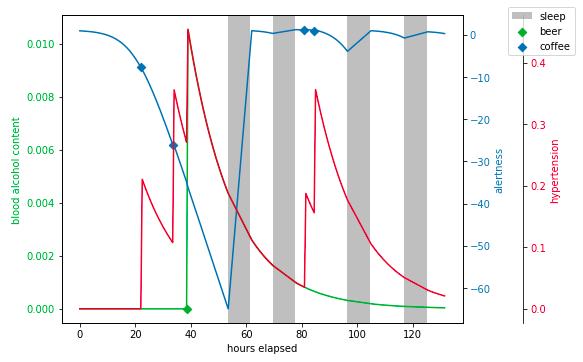
\includegraphics[width=\linewidth]{images/heartpole_example.png}
      \caption{random agent's health indicators}
      \label{fig:random}
    \end{subfigure}
    \begin{subfigure}{0.48\linewidth}
      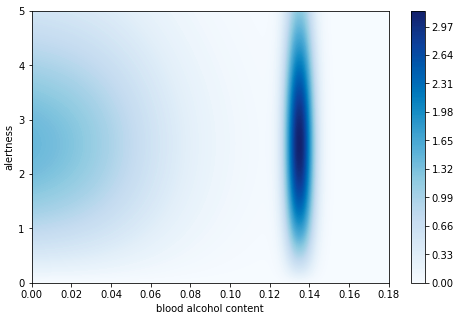
\includegraphics[width=\linewidth]{images/productivity.png}
      \caption{productivity function}
      \label{fig:productivity}
    \end{subfigure}
    \caption{HeartPole model. Not for clinical use.}
\end{figure}

We introduce a patient simulator inspired by \emph{CartPole} \cite{cartpole} that trades clinical accuracy off for \emph{simplicity} and \emph{transparency}, while still being \emph{non-trivial} to solve.

\emph{HeartPole} simulates a creative professional trying to become more productive.
However, many decisions that would help in the short term (not sleeping, consuming coffee and alcohol) can create long-term health issues that negate all short term gains.

\emph{HeartPole} is a fully observable Markov Decision Process \cite{mdp} where state $\state_\step$ consists of alertness $\state^\text{alert}_\step$, hypertension $\state^\text{hypert}_\step$, intoxication $\state^\text{tox}_\step$ time since slept $\state^\text{tawake}_\step$, \emph{total time elapsed} $\state^\text{ttotal}_\step$ and \emph{total work done} $\state^\text{done}_\step$.

Over these parameters, we define \emph{productivity} function $\eta(\state^\text{alert}_\step, \state^\text{tox}_\step)$ presented graphically on figure \ref{fig:productivity} and \emph{heart attack probability} $r(\state^\text{hypert}_\step)=\frac{\text{sigmoid}(\state^\text{hypert}_\step)}{2}$.
The agent receives small positive rewards for productivity and a very large negative reward if a heart attack occurs.

Every half an hour awake, the agent observes $\state_\step$ and picks an action $\action_\step$ from discrete action space of \emph{just work}, \emph{drink coffee} (increases $\state^\text{alert}$ and $\state^\text{hypert}$), \emph{drink beer} (decreases $\state^\text{alert}$, increases $\state^\text{hypert}$ and $\state^\text{tox}_\step$) and \emph{go to bed} (sleep takes a lot of time, but reduces $\state^\text{hypert}$ and $\state^\text{tox}_\step$ and without it alertness starts to fall very fast)

\newpage
\section{Experimental design}
\label{sec:heartpole-experiments}

We compare 3 different approaches to develop a HeartPole agent: manual programming, automatic programming and deep reinforcement learning.
Training procedure depends on the approach, while testing procedure is the same: calculating total return $\returntot$ average over 20 re-runs, limiting all episodes to 1000 steps.

\subsection{Reinforcement Learning baseline}
To make sure that the reinforcement learning baseline does not turned out to be unfairly weak due to the wrong choice of model or algorithm, we train 2 models (a neural network with 0 hidden layers against one with 3 hidden layers of size 16) each with 3 different industry-standard algorithms: CEM \cite{szitaLearningTetrisUsing2006}, SARSA \cite[Chapter 6]{suttonReinforcementLearningSecond2018} and DQN \cite{mnihPlayingAtariDeep2013,dqn}.
All models are trained with \texttt{keras-rl} \cite{KerasrlKerasrlDeep2025}. 

\subsection{Vadim baseline}

For our first baseline, we employ an expert\footnote{the author of the present thesis} to write a maximally simple reference implementation of a HeartPole agent.
The resulting code is as follows:

\lstinputlisting{listings/metanurse-vadim.py}

\newpage
\subsection{Program Synthesis}

\begin{table}
    \centering
    \begin{tabular}{|c|c|c|c|c|c|}
        model & $\treearity_\text{draft}$ & $\treearity_\text{explain}$ & $\treearity_\text{debug}$ & $\beamwidth$ & selection \\
        \midrule
        gpt-4o & 3 & 2 & 2 & 5 & tournament \\
        deepseek-coder & 3 & 2 & 2 & 5 & tournament
    \end{tabular}
    \caption{Hyperparameter choice for evaluating RLCEPS on HeartPole}
    \label{tab:rlceps-heartpole}
\end{table}

We use the best performing Reinforcement Learning from Code Execution Feedback (RLCEF) approach discovered in part \ref{part:proginduction}, namely SEIDR (chapter \ref{ch:seidr}) with hyperparameters presented in table \ref{tab:rlceps-heartpole}, 2 different recently released and strongly benchmarked language models (GPT-4o~\cite{openaiGPT4oSystemCard2024} and DeepSeek Coder~\cite{guoDeepSeekCoderWhenLarge2024}) and the following initial prompt: 

\lstinputlisting{listings/metaheartpole_prompt.txt}

Note that this prompt does not include any information about the model HeartPole uses, such as the productivity function or heart attack probability.
Thus, all the important information about the environment has to be disovered by SEDIR via trial and error.
This approach lets use model the use of program synthesis for scientific discovery as discussed in section \ref{sec:scientific-discovery}: how much could we learn about the environment by exploring the programs that were optimized to thrive in it?

\newpage
\section{Results}

DeepSeek turned out to be the only algorithm with a taste for beer:

\lstinputlisting{listings/metanurse-deepseek.py}

GPT came up with a more conservative algorithm, similar to the Vadim baseline:

\lstinputlisting{listings/metanurse-gpt.py}

\begin{table}[]
    \centering
    \begin{tabular}{lrr}
\toprule
model & avg score & best avg score \\
\midrule
deepseek-coder & -149.952560 & 0.400517 \\
gpt-4o & -99.885775 & 0.348758 \\
\bottomrule
\end{tabular}
    \caption{Summary of HeartPole agents: which actions they used and final scores}
    \label{tab:heartpole-results}
\end{table}


Table \ref{tab:heartpole-results} summarizes the results of our experiment. Overall, we can conclude that

\begin{enumerate}
    \item The best result is achieved by a deep reinforcement learning model using DQN algorithm.
    Selecting a program synthesis approach solely for performance benefits might be unwise.
    \item At the same time, performance of different approaches is very similar.
    \item Program synthesis can indeed be a powerful tool for scientific discovery: the resulting programs are highly interpretable and interesting.
\end{enumerate}